% ------------------------------------------------------------------------
% ------------------------------------------------------------------------
% abnTeX2: Modelo de Trabalho Academico (tese de doutorado, dissertacao de
% mestrado e trabalhos monograficos em geral) em conformidade com 
% ABNT NBR 14724:2011: Informacao e documentacao - Trabalhos academicos -
% Apresentacao
% ------------------------------------------------------------------------
% ------------------------------------------------------------------------

% ------------------------------------------------------------------------
% ------------------------------------------------------------------------
% abnTeX2: Modelo de Trabalho Academico (tese de doutorado, dissertacao de
% mestrado e trabalhos monograficos em geral) em conformidade com 
% ABNT NBR 14724:2011: Informacao e documentacao - Trabalhos academicos -
% Apresentacao
% ------------------------------------------------------------------------
% ------------------------------------------------------------------------

\documentclass[
	% -- opções da classe memoir --
	12pt,				% tamanho da fonte
	openright,			% capítulos começam em pág ímpar (insere página vazia caso preciso)
	oneside,			% para impressão em verso e anverso. Opções: oneside/twoside
	a4paper,			% tamanho do papel. 
	% -- opções da classe abntex2 --
	%chapter=TITLE,		% títulos de capítulos convertidos em letras maiúsculas
	%section=TITLE,		% títulos de seções convertidos em letras maiúsculas
	%subsection=TITLE,	% títulos de subseções convertidos em letras maiúsculas
	%subsubsection=TITLE,% títulos de subsubseções convertidos em letras maiúsculas
	% -- opções do pacote babel --
	english,			% idioma adicional para hifenização
	french,				% idioma adicional para hifenização
	spanish,			% idioma adicional para hifenização
	brazil				% o último idioma é o principal do documento
	]{abntex2}

	% ---
	% Pacotes básicos 
	% ---
	\usepackage{lmodern}			% Usa a fonte Latin Modern			
	\usepackage[T1]{fontenc}		% Selecao de codigos de fonte.
	\usepackage[utf8]{inputenc}		% Codificacao do documento (conversão automática dos acentos)
	\usepackage{lastpage}			% Usado pela Ficha catalográfica
	\usepackage{indentfirst}		% Indenta o primeiro parágrafo de cada seção.
	\usepackage{color}			% Controle das cores
	\usepackage{graphicx}			% Inclusão de figuras
	\usepackage{microtype} 			% para melhorias de justificação
	\usepackage{epsfig,psfrag,amsmath,tabularx} % para figuras eps e simbolos matematicos
	\graphicspath{{capitulos/imagens/}}
% ---

% ---
% Pacotes de citações
% ---
\usepackage[brazilian,hyperpageref]{backref}	 % Paginas com as citações na bibl
\usepackage[alf]{abntex2cite}			 % Citações padrão ABNT

% --- 
% CONFIGURAÇÕES DE PACOTES 
% --- 

% ---
% Configuracoes do pacote backref
% Usado sem a opcao hyperpageref de backref
\renewcommand{\backrefpagesname}{Citado na(s) página(s):~}
% Texto padrao antes do numero das paginas
\renewcommand{\backref}{}
% Define os textos da citacao
\renewcommand*{\backrefalt}[4]{
	\ifcase #1 %
		Nenhuma citação no texto.%
	\or
		Citado na página #2.%
	\else
		Citado #1 vezes nas páginas #2.%
	\fi}%
% ---

% ---
% Pacotes definidos pelo autor
% ---
\input{macros}		% arquivo com possiveis macros definidas pelo autor
% ---

% ---
% Informacoes de dados para CAPA e FOLHA DE ROSTO
% ---
\titulo{DOCUMENTAÇÃO DA ENTREGA INTERMEDIÁRIA\\“Aplicativo para gerência/compartilhamento de contas da mesa”}
\autor{Abner Cleto Filho\\Anderson Bernardo de Almeida\\Rafael Henrique da Silva Correia\\Vitor Talaia de Oliveira}
\local{Sorocaba, SP}
\data{29 de Setembro de 2016}

% ---
%\orientador{Prof. Dr. nome do orientador}
%\coorientador{Prof. Dr. nome do coorientador}
% ---

\instituicao{%
  Universidade Federal de São Carlos -- UFSCar
  \par
  Centro de Ciências em Gestão e Tecnologia -- CCGT
  \par
  Programa de Pós-Graduação em Ciência da Computação -- PPGCC-So}

\tipotrabalho{Dissertação (Mestrado)}
% O preambulo deve conter o tipo do trabalho, o objetivo, 
% o nome da instituicao e a Area de concentracao 
\preambulo{Documentação referente à primeira fase do projeto “Aplicativo para gerência/compartilhamento de contas da mesa”, desenvolvido pelo Grupo XXX, apresentado para a disciplina de “Tópicos em Interface Humano-computador”, ministrada pela Prof.ª Dr.ª Luciana Martinez Zaina.}
% ---


% ---
% Configuracoes de aparencia do PDF final

% alterando o aspecto da cor azul
\definecolor{blue}{RGB}{41,5,195}

% informacoes do PDF
\makeatletter
\hypersetup{
     	%pagebackref=true,
	pdftitle={\@title}, 
	pdfauthor={\@author},
    	pdfsubject={\imprimirpreambulo},
	pdfcreator={LaTeX with abnTeX2},
	pdfkeywords={abnt}{latex}{abntex}{abntex2}{trabalho acadêmico}, 
	colorlinks=true,       		% false: boxed links; true: colored links
    	linkcolor=blue,          	% color of internal links
    	citecolor=blue,        		% color of links to bibliography
    	filecolor=magenta,      	% color of file links
	urlcolor=blue,
	bookmarksdepth=4
}
\makeatother
% --- 

% --- 
% Espacamentos entre linhas e paragrafos 
% --- 

% O tamanho do paragrafo é dado por:
\setlength{\parindent}{1.3cm}

% Controle do espaçamento entre um parágrafo e outro:
\setlength{\parskip}{0.2cm}  % tente também \onelineskip

% ---
% compila o indice
% ---
\makeindex
% ---




% ----
% Inicio da dissertacao
% ----
\begin{document}

% Retira espaco extra obsoleto entre as frases.
\frenchspacing


% ----------------------------------------------------------
% ELEMENTOS PRE-TEXTUAIS
% ----------------------------------------------------------
% \pretextual

% ---
% Capa
% ---
\imprimircapa
% ---

% ---
% Folha de rosto
% (o * indica que havera a ficha bibliografica)
% ---
\imprimirfolhaderosto
% ---

% ---
% Inserir a ficha bibliografica		--> Comentado por Anderson
% ---
%\input{pretextuais/1-fichaCatalografica.tex}
% ---

% ---
% Inserir folha de aprovacao		--> Comentado por Anderson
% ---
%\input{pretextuais/2-folhaAprovacao.tex}
% ---

% ---
% Dedicatoria				--> Comentado por Anderson
% ---
%\input{pretextuais/3-dedicatoria}
% ---

% ---
% Agradecimentos			--> Comentado por Anderson
% ---
%\input{pretextuais/4-agradecimento}
% ---

% ---
% Epigrafe				--> Comentado por Anderson
% ---
%\input{pretextuais/5-epigrafe}
% ---

% ---
% RESUMOS
% ---
%================================= Resumo e Abstract ========================================
\setlength{\absparsep}{18pt} % ajusta o espaçamento dos paragrafos do resumo 
                     
% --- 
% resumo em português
% --- 
\begin{resumo}

Escrever o resumo aqui.

\textbf{Palavras-chaves}: Palavra1. Palavra2. Palavra3.

\end{resumo}
% --- 


% --- 
% resumo em ingl�s
% --- 
\begin{resumo}[Abstract]
 \begin{otherlanguage*}{english}

Write the abstract here.

\textbf{Key-words}: Word1. Word2. Word3.

 \end{otherlanguage*}
\end{resumo}
% --- 

%===========================================================================================

% ---


%=============================== lista de figuras ==========================
\pdfbookmark[0]{\listfigurename}{lof}
\listoffigures*
\cleardoublepage


%=============================== lista de tabelas ==========================
\pdfbookmark[0]{\listtablename}{lot}
\listoftables*
\cleardoublepage


%====================== lista de abreviaturas e siglas =====================
\input{pretextuais/7-abreviaturas.tex}


%============================ lista de simbolos ============================
\input{pretextuais/8-simbolos.tex}


%=============================== sumario =============================================
\pdfbookmark[0]{\contentsname}{toc}
\tableofcontents*
\cleardoublepage


% ----------------------------------------------------------
% AQUI INICIA OS ELEMENTOS DO TEXTO
% ----------------------------------------------------------
\textual

\chapter*[Introdução]{Introdução}
\addcontentsline{toc}{chapter}{Introdução}


Com a popularização dos dispositivos móveis hoje parte integrante da vida de grande parte da população, o mercado de tecnologia teve grande foco no desenvolvimento de aplicativos que pudessem auxiliar em atividades recorrentes das pessoas, tornando processos anteriormente manuais, automatizados; visando sempre a agilidade, segurança e conforto ao usuário.
Neste contexto, diversas aplicações surgiram e dentre elas os aplicativos de gerenciamento de contas tem se tornado um grande atrativo para o público, seja um aplicativo voltado para um gerenciamento de longo ou curto prazo, tais aplicativos visam eliminar a necessidade de papéis e/ou informações guardadas e processadas pelo nosso cérebro.
Entretanto, assim como outros aplicativos, muitas questões podem ser esquecidas ou tratadas com irresponsabilidade durante a construção da aplicação, dentre elas as questões relacionadas à própria Interação Humano-Computador (IHC), assunto altamente debatido e analisado na atual era da informação.
É neste cenário que o presente documento visa analisar dois aplicativos com a finalidade de gerência/compartilhamento de contas da mesa comumente usado entre amigos que saem em grupo a fim de fazer um “happy hour”. Ao final desta análise propomos uma nova aplicação que vise suprir as necessidades encontradas nos aplicativo analisados, sendo os dados coletados a partir de um grupo de usuários conforme descrito neste documento.

\chapter{Escopo}\label{cap1}

O escopo do projeto é delimitado pelos seguintes fatores:

% ---
\section{Propósito}
% ---

O aplicativo proposto tem a finalidade de proporcionar o gerenciamento e o compartilhamento da conta de uma mesa em um estabelecimento alimentício, onde pessoas que o visitem em grupo possam compartilhar a conta e gerenciá-las individualmente ou em grupo, podendo assim realizar o controle da divisão dos pedidos e dos gastos da mesa em tempo real, sendo as informações do aplicativo providenciadas pelos próprios usuários.
\chapter{Sistemas Semelhantes}\label{cap2}

Vários aplicativos com a finalidade apresentada encontram-se disponíveis atualmente, dentre estes foram escolhidos os seguintes para ser realizada a análise de IHC, apresentada no próximo tópico.

\section{Aplicativo ``PassaRégua''}

Disponível no seguinte endereço:

https://play.google.com/store/apps/details?id=passaregua.first.android

Descrição: “O Aplicativo Passa Régua tem como objetivo permitir você dividir contas de maneira prática, consistente e com um visual semelhante ao famoso cupom fiscal que recebemos com o valor de nossa conta nos restaurantes e bares do Brasil.
Em poucos toques você será capaz de dividir o valor total da sua conta com seu grupo de amigos podendo inserir ou remover a taxa de serviço geralmente cobrada em alguns lugares, além disso é possível separar na divisão aquelas pessoas que consomem bebidas ou itens caros que tornam injusto a divisão por igual. Tudo isso de forma fácil e rápida, tornando possível a divisão correta até mesmo para aqueles que bebem um pouquinho a mais.” (iOasys, GooglePlay)
\include{capitulos/4-cap3}
\chapter{Capítulo de Testes}\label{cap4}

Este capítulo apresenta diversos testes em \LaTeX.
Deverá ser removido ao final (Anderson).

\section{Citações}

Teste de Citação direta com mais de 3 linhas:

\begin{citacao}
As citações diretas, no texto, com mais de três linhas, devem ser
destacadas com recuo de 4 cm da margem esquerda, com letra menor que a do texto
utilizado e sem as aspas. No caso de documentos datilografados, deve-se
observar apenas o recuo \cite[5.3]{NBR10520:2002}.
\end{citacao}


Outras citações:

É amplamente sabido e divulgado que esta linha encontra-se neste local apenas para ocupar espaço \cite{van86}.

De forma análoga, \citeonline{macedo2005} diz que ``Batatinha quando nasce se esparrama pelo chão, menininha quando dorme, põe a mão no coração''. 

Note que em \LaTeX, as aspas iniciais e finais \emph{no código} são diferentes, mas no texto compilado elas se apresentam como aspas inglesas.



\section{Figuras}


\begin{figure}[h]
	\caption{\label{fig_app}Aplicativo A}
	\begin{center}
	    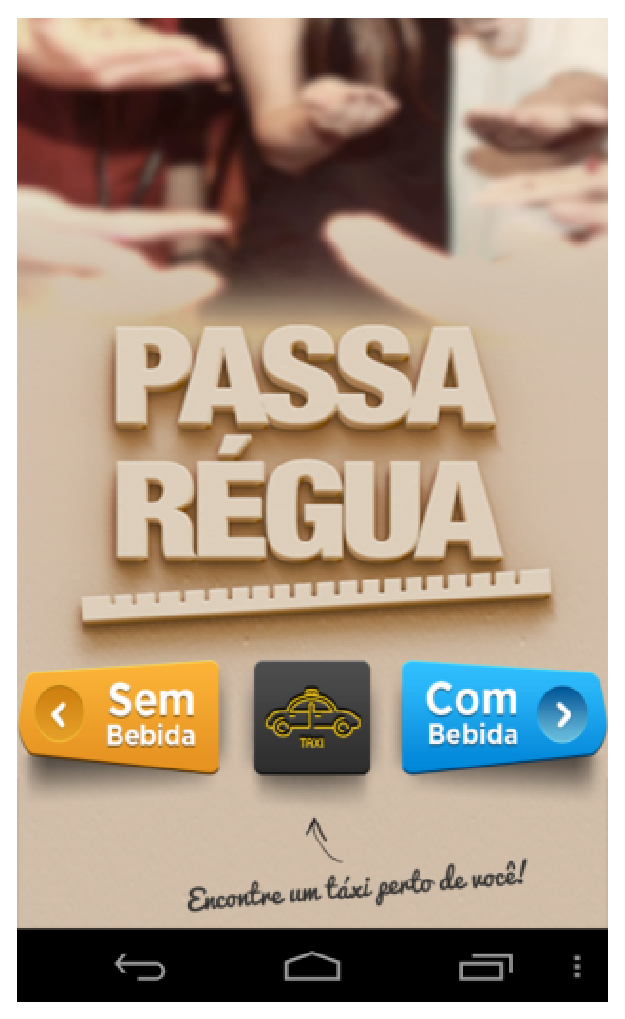
\includegraphics[scale=0.3]{image1}
	\end{center}
	\legend{Fonte: \citeonline[p. 24]{araujo2012}}
\end{figure}



% ---
\section{Expressões matemáticas}
% ---

\index{expressões matemáticas}Use o ambiente \texttt{equation} para escrever
expressões matemáticas numeradas:

\begin{equation}
  \forall x \in X, \quad \exists \: y \leq \epsilon
\end{equation}

Escreva expressões matemáticas entre \$ e \$, como em $ \lim_{x \to \infty}
\exp(-x) = 0 $, para que fiquem na mesma linha.


\include{capitulos/5-conclusao}
% ---------------------------------------------------------- 

% ----------------------------------------------------------
% ELEMENTOS POS-TEXTUAIS
% ----------------------------------------------------------
\postextual
% ----------------------------------------------------------

% ----------------------------------------------------------
% Referencias bibliograficas
% ----------------------------------------------------------
\bibliography{referencias}


% ----------------------------------------------------------
% Glossario
% ----------------------------------------------------------
%
% Consulte o manual da classe abntex2 para orientacoes sobre o glossario.
%
%\glossary

% ----------------------------------------------------------
% Apendices
% ----------------------------------------------------------

% ---
% Inicia os apendices
% ---
\begin{apendicesenv}

\include{capitulos/6-apendice1}

\end{apendicesenv}
% ---

% ----------------------------------------------------------
% Anexos
% ----------------------------------------------------------

% ---
% Inicia os anexos
% ---
\begin{anexosenv}

\include{capitulos/7-anexo1}

\end{anexosenv}
% --- 

%---------------------------------------------------------------------
% INDICE REMISSIVO
%---------------------------------------------------------------------
\phantompart
\printindex
%---------------------------------------------------------------------

\end{document}
